% Suggested replacements for the empty numerical subsections in the supplied
% manuscript. Place at repository root or adjust the itw2027/ relative paths.
% This is a results fragment, not a full manuscript; review final page count.

\subsection{Numerical Results}
\label{sec:noiseless_numerical}
We evaluate identification ($S=1$), the rank test
$f(i)=\1\{\operatorname{int}(i)\leq20\}$ ($S=21$), and the exact-threshold
test $f(i)=\1\{\|i\|_1=2\}$ ($S=\binom{m}{2}$). For
$n_t\in\{24,26,\ldots,40\}$ and $E_2=0.1$, we set $r=n_t/2$, $T=2^r$,
and $m=rK$, with the largest $K$ satisfying
$K S_{\rm up}(rK)\leq2^{n_t(1/2-E_2)}$, where $S_{\rm up}=S$ for
identification and rank, and $S_{\rm up}(m)=m^2/2$ is a conservative
envelope for the exact-threshold support. The finite rate is
$R_t=\log_2(m)/n_t$. For each setting, we sample $2{,}000$ negative
messages ($200$ for identification at $n_t=38,40$) and enumerate all $T$
RS positions, giving the exact conditional FP probability of each sampled
message; FN is zero by construction.

Fig.~\ref{fig:itw27_noiseless}(a) directly checks
Proposition~\ref{prop:finite_error}: every sampled FP probability is below
$B=S(K-1)/T$. At $n_t=40$, the sampled maxima are
$3.81\times10^{-6}$, $3.62\times10^{-5}$, and $7.04\times10^{-3}$ for
identification, rank, and exact threshold, respectively, versus bounds
$0.0625$, $0.0625$, and $0.0340$, showing that the uniform guarantee can be
conservative for these functions. Separately, $22$ tested arbitrary
supports attain $B$ exactly; this confirms tightness for those unrestricted
supports, not for the named rank and threshold functions.
Fig.~\ref{fig:itw27_noiseless}(b) deterministically evaluates the certified
design. With fixed $E_2=0.1$, the rates approach $0.4$
for constant weights and $2/15$ for $\beta=2$; with
$E_2(n_t)=n_t^{-1/2}$, the bound $2^{-\sqrt{n_t}}$ vanishes while the rates
approach the asymptotic benchmarks $1/2$ and $1/6$. Finite-length
prefactors explain values above a benchmark at small $n_t$.

\begin{figure}[t]
  \centering
  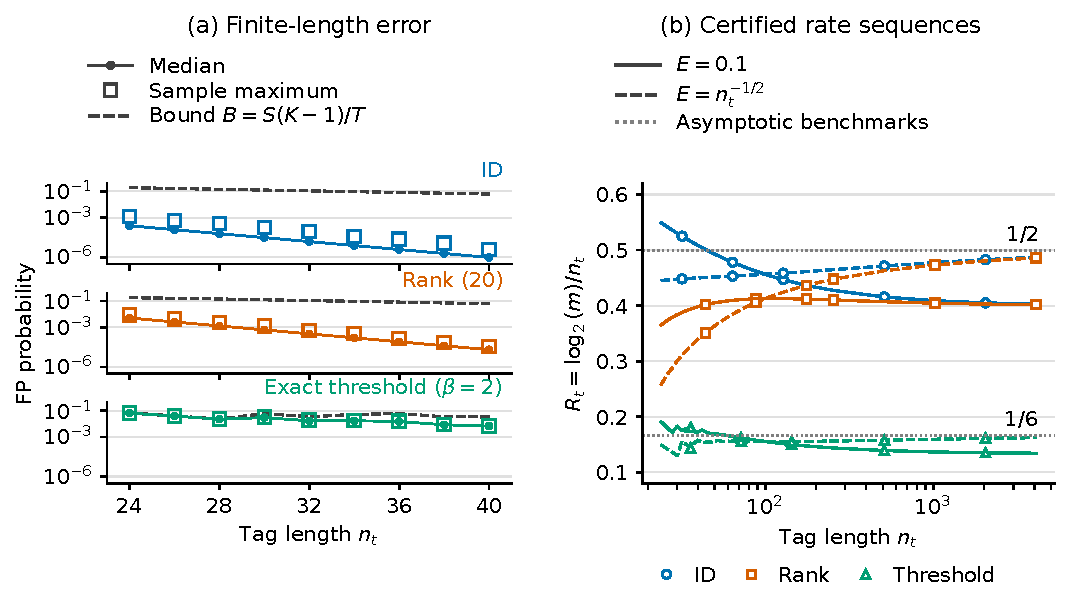
\includegraphics[width=\columnwidth]{itw2027/results/processed/figures/figure1_noiseless.pdf}
  \caption{Noiseless RS tagging: (a) sampled conditional FP probabilities and uniform bounds; (b) certified finite rates and asymptotic benchmarks.}
  \label{fig:itw27_noiseless}
\end{figure}

% Insert in the noisy-channel section, replacing its empty subsection.
\subsection{Numerical Results}
\label{sec:noisy_numerical}
We concatenate the tags with a rate-$1/2$ normal-frame DVB-S2 LDPC code
($N_b=64{,}800$, $N_i=32{,}400$), transmit BPSK over AWGN, and use
belief-propagation decoding with early termination and at most $50$
iterations. The sweep uses $E_b/N_0=0.5,0.6,\ldots,2.6$ dB and $2{,}500$
frames per point, where $E_b$ is normalized per occupied payload bit. A
fixed, balanced bank of positive and negative examples is reused across
SNRs for each function, so FP and FN are class-conditional; frames, rather
than packed tags, are the sampling units for channel-error uncertainty.
All functions use $E_2=0.1$ and $n_t=40$, giving $G=810$ tags per frame
without padding, $n_{\rm eff}=N_b/G=80$, and
$R_{\rm eff}=G\log_2(m)/N_b$ (Table~\ref{tab:itw27_parameters}). This rate
is amortized; each decision still requires decoding the full LDPC frame.

Fig.~\ref{fig:itw27_noisy}(a) shows the LDPC waterfall and the resulting
channel-induced FN events. At every plotted point, each payload-correct
frame reproduces its paired noiseless decisions, and every FN is confined
to a payload-error frame. This verifies the simulated error-event
decomposition behind Proposition~\ref{prop:noisy_finite_error}, including
the absence of a factor $G$ in an individual task's bound. As payload FER falls,
Fig.~\ref{fig:itw27_noisy}(b) shows FP approaching the corresponding
noiseless collision floor. At $1.5$ dB, no payload errors or FNs occur in
$2{,}500$ frames, while FP is $2.96\times10^{-6}$, $2.47\times10^{-5}$,
and $6.81\times10^{-3}$ for identification, rank, and exact threshold.
The dashed $\min\{1,B+\widehat{\mathrm{FER}}\}$ curves visualize the
additive structure but are not rigorous theorem bounds: the empirical
payload FER is not the maximal $\xi$ assumed by the proposition. Nor do
zero observed failures imply zero error; their one-sided $95\%$ frame-level
upper limit is $1.20\times10^{-3}$.

\begin{table}[t]
  \centering
  \caption{Implemented configurations with $N_b=64{,}800$,
  $N_i=32{,}400$, and inner design $E_2=0.1$; $m$ is the message length
  in bits, and rates use exponential message-length scaling.}
  \label{tab:itw27_parameters}
  \normalsize
  \setlength{\tabcolsep}{2pt}
  \begin{tabular}{lrrrrrr}
\hline
Function & $n_t$ & $m$ & $S$ & $R_t$ & $G$ & $R_{\rm eff}$\\
\hline
ID & 40 & 1,310,720 & 1 & 0.508 & 810 & 0.254\\
Rank (20) & 40 & 62,400 & 21 & 0.398 & 810 & 0.199\\
Exact ($\beta=2$) & 42 & 168 & 14,028 & 0.176 & 771 & 0.088\\
\hline
\end{tabular}

\end{table}

\begin{figure}[t]
  \centering
  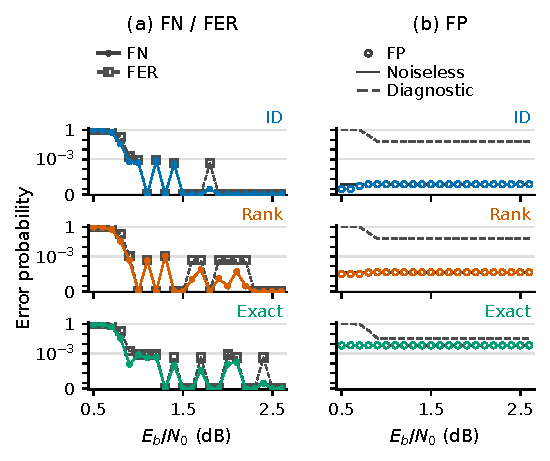
\includegraphics[width=\columnwidth]{itw2027/results/processed/figures/figure2_noisy.pdf}
  \caption{Packed BFC over AWGN: (a) channel-induced FN and payload FER; (b) conditional FP, paired noiseless reference, and empirical additive diagnostic.}
  \label{fig:itw27_noisy}
\end{figure}
